\documentclass[tikz,border=2pt]{standalone}
\usepackage{amsmath}
\usepackage{pgfplots}
\pgfplotsset{compat=1.18}

\begin{document}
% The principal n-th root undoes x -> x^n on [0,∞): sqrt(x) is the mirror image of x^2 (x>=0)
% in the line y=x; the cube root is defined for all real x.
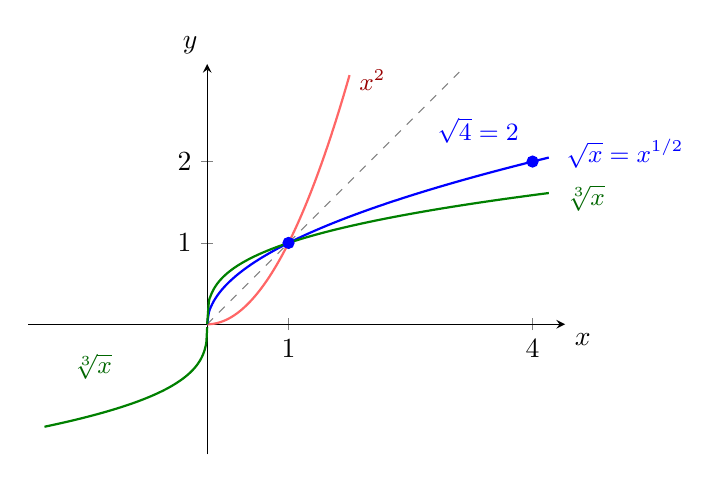
\begin{tikzpicture}
	\begin{axis}[
		axis lines=middle,
		axis equal image,
		xmin=-2.2, xmax=4.4,
		ymin=-1.6, ymax=3.2,
		xtick={1,4}, ytick={1,2},
		xlabel={$x$}, ylabel={$y$},
		xlabel style={below right}, ylabel style={above left},
		samples=200, smooth, clip=false,
		width=8.4cm
		]
		\addplot[gray, dashed, domain=0:3.1] {x};
		\addplot[thick, red!60, domain=0:1.75] {x^2};
		\addplot[thick, blue, domain=0:4.2] {sqrt(x)};
		\addplot[thick, green!50!black, domain=0:4.2] {x^(1/3)};
		\addplot[thick, green!50!black, domain=-2:0] {-(-x)^(1/3)};
		\addplot[only marks, mark=*, blue] coordinates {(4,2) (1,1)};
		\node[blue, anchor=west, font=\small] at (axis cs:4.3,2.1) {$\sqrt{x}=x^{1/2}$};
		\node[red!60!black, anchor=west, font=\small] at (axis cs:1.75,3.0) {$x^2$};
		\node[green!40!black, anchor=south east, font=\small] at (axis cs:-1.05,-0.8) {$\sqrt[3]{x}$};
		\node[green!40!black, anchor=west, font=\small] at (axis cs:4.3,1.55) {$\sqrt[3]{x}$};
		\node[blue, anchor=south east, font=\small] at (axis cs:3.95,2.1) {$\sqrt4=2$};
	\end{axis}
\end{tikzpicture}
\end{document}
